%(BEGIN_QUESTION)
% Copyright 2011, Tony R. Kuphaldt, released under the Creative Commons Attribution License (v 1.0)
% This means you may do almost anything with this work of mine, so long as you give me proper credit

En operatør hevder at dette flow-reguleringssystemet ikke regulerer prosessflow korrekt. Selv om PV på regulatorfronten er lik SP (begge viser 386 GPM i område 0--500 GPM), mener operatøren at faktisk flow er langt lavere (omtrent 220 GPM), basert på massebalanseberegninger i et nedstrøms prosessledd. Du legger også merke til at regulatorutgangen står på 35\%:

$$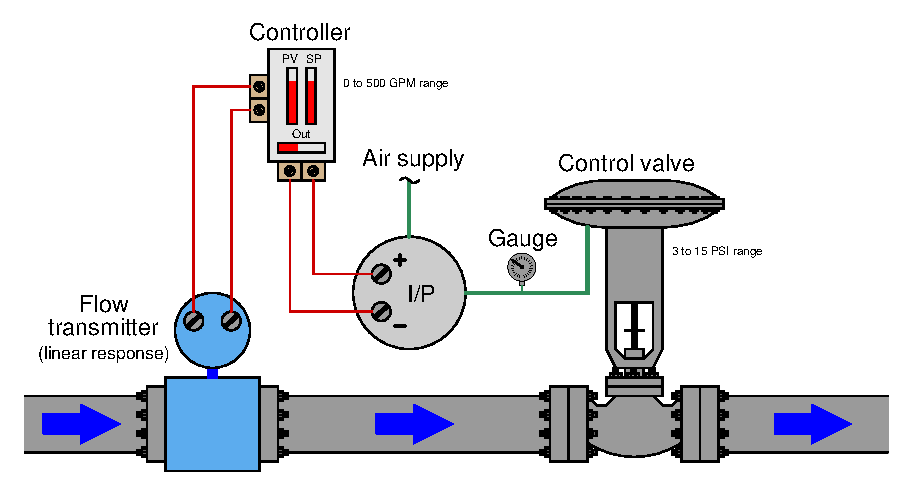
\includegraphics[width=15.5cm]{i00362x01.eps}$$

Første test er å måle sløyfestrøm i kretsen mellom flowtransmitter og flowregulator. Multimeteret viser 11.05 mA. Neste steg er å lese av trykkmåleren: 7 PSI.

\vskip 10pt

Vurder sannsynligheten for hver oppgitt feil i dette reguleringssystemet. Se på én feil om gangen (ingen sammenfallende feil), og avgjør om hver feil alene kan forklare {\it alle} målinger og symptomer i kretsen.

% No blank lines allowed between lines of an \halign structure!
% I use comments (%) instead, so that TeX doesn't choke.

$$\vbox{\offinterlineskip
\halign{\strut
\vrule \quad\hfil # \ \hfil & 
\vrule \quad\hfil # \ \hfil & 
\vrule \quad\hfil # \ \hfil \vrule \cr
\noalign{\hrule}
%
% First row
{\bf Feil} & {\bf Mulig} & {\bf Umulig} \cr
%
\noalign{\hrule}
%
% Another row
FT ute av kalibrering (sender feil strøm) &  &  \cr
%
\noalign{\hrule}
%
% Another row
FIC-inngang ute av kalibrering (tolker signal feil) &  &  \cr
%
\noalign{\hrule}
%
% Another row
FIC-utgang ute av kalibrering (sender feil mA-signal til I/P) &  &  \cr
%
\noalign{\hrule}
%
% Another row
Trykkmåler ute av kalibrering (viser feil trykk) &  &  \cr
%
\noalign{\hrule}
%
% Another row
I/P ute av kalibrering (gir feil trykk ut) &  &  \cr
%
\noalign{\hrule}
%
% Another row
Reguleringsventilen er overdimensjonert &  &  \cr
%
\noalign{\hrule}
%
% Another row
Reguleringsventilen er underdimensjonert &  &  \cr
%
\noalign{\hrule}
%
% Another row
Ventilens bench-set er feiljustert &  &  \cr
%
\noalign{\hrule}
%
% Another row
FIC er dårlig trimmet &  &  \cr
%
\noalign{\hrule}
%
% Another row
Operatørens massebalanseberegninger er feil &  &  \cr
%
\noalign{\hrule}
} % End of \halign 
}$$ % End of \vbox

\underbar{file i00362}
%(END_QUESTION)





%(BEGIN_ANSWER)

% No blank lines allowed between lines of an \halign structure!
% I use comments (%) instead, so that TeX doesn't choke.

$$\vbox{\offinterlineskip
\halign{\strut
\vrule \quad\hfil # \ \hfil & 
\vrule \quad\hfil # \ \hfil & 
\vrule \quad\hfil # \ \hfil \vrule \cr
\noalign{\hrule}
%
% First row
{\bf Feil} & {\bf Mulig} & {\bf Umulig} \cr
%
\noalign{\hrule}
%
% Another row
FT ute av kalibrering (sender feil strøm) &  & $\surd$ \cr
%
\noalign{\hrule}
%
% Another row
FIC-inngang ute av kalibrering (tolker signal feil) & $\surd$ &  \cr
%
\noalign{\hrule}
%
% Another row
FIC-utgang ute av kalibrering (sender feil mA-signal til I/P) &  & $\surd$ \cr
%
\noalign{\hrule}
%
% Another row
Trykkmåler ute av kalibrering (viser feil trykk) &  & $\surd$ \cr
%
\noalign{\hrule}
%
% Another row
I/P ute av kalibrering (gir feil trykk ut) &  & $\surd$ \cr
%
\noalign{\hrule}
%
% Another row
Reguleringsventilen er overdimensjonert &  & $\surd$ \cr
%
\noalign{\hrule}
%
% Another row
Reguleringsventilen er underdimensjonert &  & $\surd$ \cr
%
\noalign{\hrule}
%
% Another row
Ventilens bench-set er feiljustert &  & $\surd$ \cr
%
\noalign{\hrule}
%
% Another row
FIC er dårlig trimmet &  & $\surd$ \cr
%
\noalign{\hrule}
%
% Another row
Operatørens massebalanseberegninger er feil &  & $\surd$ \cr
%
\noalign{\hrule}
} % End of \halign 
}$$ % End of \vbox

%(END_ANSWER)





%(BEGIN_NOTES)

{\bf Denne oppgaven er ment for eksamen og ikke for arbeidsark!}.

%(END_NOTES)
